\documentclass[12pt, twoside]{article}
\usepackage[letterpaper, margin=1in, headsep=0.5in]{geometry}
\usepackage[english]{babel}
\usepackage[utf8]{inputenc}
\usepackage{amsmath}
\usepackage{amsfonts}
\usepackage{amssymb}
\usepackage{tikz}
\usetikzlibrary{quotes, angles}
\usepackage{graphicx}
\usepackage{enumitem}
\usepackage{multicol}
\usepackage{hyperref}

\newif\ifmeta
\metatrue %print standards and topics tags

\title{IB Mathematics}
\author{Chris Huson}
\date{February 2022}

\usepackage{fancyhdr}
\pagestyle{fancy}
\fancyhf{}
\renewcommand{\headrulewidth}{0pt} % disable the underline of the header
\raggedbottom


\fancyhead[LE]{\thepage}
\fancyhead[RO]{\thepage \\ Name: \hspace{4cm} \,\\}
\fancyhead[LO]{BECA / IB Math 4-Polynomial and rational functions\\* 10 February 2022}

\begin{document}

\subsubsection*{4.11 PreQuiz: Linear equations}
\begin{enumerate}
    \item A linear function $f$ is graphed below.
    \begin{multicols}{2}
    \begin{enumerate}
      \item Write down it's slope.\\ $m=$
      \vspace{0.25cm}
      \item Write down it's $y$-intercept.\\ $b=$
      \vspace{0.25cm}
      \item Write down the equation of the line.
    \end{enumerate} \vspace{.5cm}
      \begin{center} 
      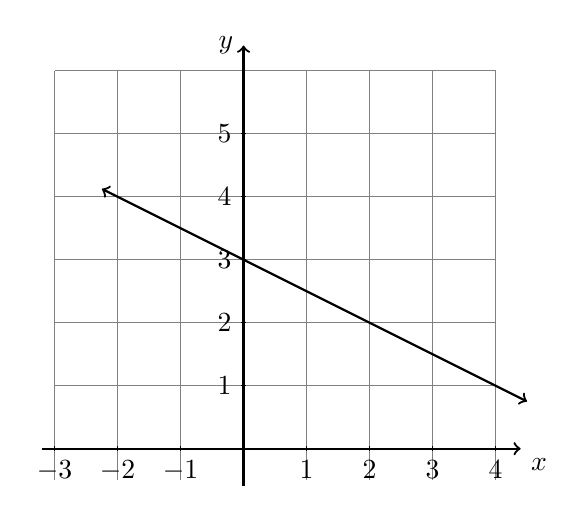
\begin{tikzpicture}[scale=0.8]
        \draw [help lines] (-3,-0.5) grid (4,6);
        \draw [thick, ->] (-3.2,0) -- (4.4,0) node [below right] {$x$};
        \draw [thick, ->] (0,-0.6)--(0,6.4) node [left] {$y$};
        \foreach \x in {-3,-2,-1,1,2,...,4} \draw (\x cm,1pt) -- (\x cm,-1pt) node[anchor=north] {$\x$};
        \foreach \y in {1, 2, 3, 4, 5} \draw (1pt,\y cm) -- (-1pt,\y cm) node[anchor=east] {$\y$};
        \draw [thick, <->,smooth,samples=20,domain=-2.25:4.5] plot(\x,-0.5*\x+3);
      \end{tikzpicture}
      \end{center}
    \end{multicols} \vspace{1cm}
    
    \item Write the linear equation $y+1=2(x-6)$ in the form $y=mx+c$. \vspace{4cm}
    
    \item A line has a gradient (slope) of $\displaystyle -\frac{3}{2}$ and passes through the point $(6, 1)$. Find the equation of the line in the form $y=mx+c$.
    
\newpage
\item A line goes through the points $(2,3)$ and $(6, -1)$. \hfill [5]
    \begin{enumerate}
      \begin{multicols}{2}
          \item Find the gradient of the line.
          \item Find the equation of the line in the form $y=mx+c$.\vspace{2cm}
          \begin{center}
          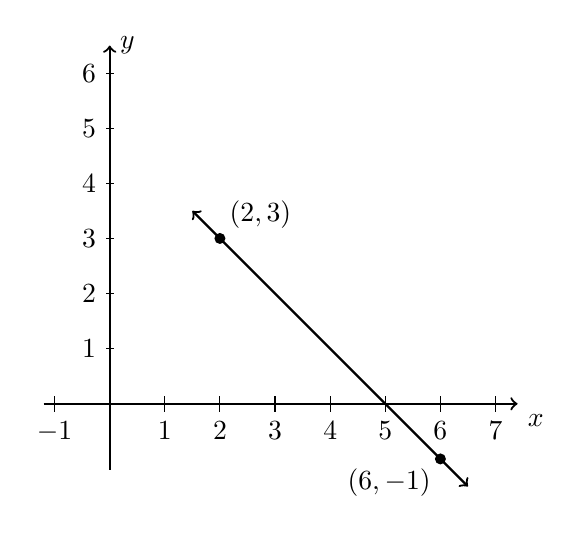
\begin{tikzpicture}[xscale=0.7, yscale=0.7]
            %\draw [help lines] (-3,-2) grid (4,6);
            \draw [thick, ->] (-1.2,0) -- (7.4,0) node [below right] {$x$};
            \draw [thick, ->] (0,-1.2)--(0,6.5) node [right] {$y$};
            \foreach \x in {-1, 1,2, ...,7} \draw (\x cm,4pt) -- (\x cm,-4pt) node[anchor=north] {$\x$};
            \foreach \y in {1,2,...,6} \draw (2pt,\y cm) -- (-2pt,\y cm) node[anchor=east] {$\y$};
            \fill (2,3) circle[radius=0.1] node[above right]{$(2,3)$};
            \fill (6,-1) circle[radius=0.1] node[below left]{$(6,-1)$};
            \draw [thick, <->,smooth,samples=20,domain=1.5:6.5] plot(\x,-1.0*\x+5);
          \end{tikzpicture}
          \end{center}
        \end{multicols}
    \end{enumerate} \vspace{2.cm}
    
\item A linear equation is desired to model a set of data.
\begin{enumerate}
    \item Plot the following points on the grid: $(-4,2)$, $(-3,1)$, $(-1,2)$, $(1,4)$, $(3,5)$, $(5,5)$
    \item Draw a line of best fit through the data. (use a straight edge for full credit)
    \item Write down the equation of the line.
\end{enumerate}
    \begin{center}
        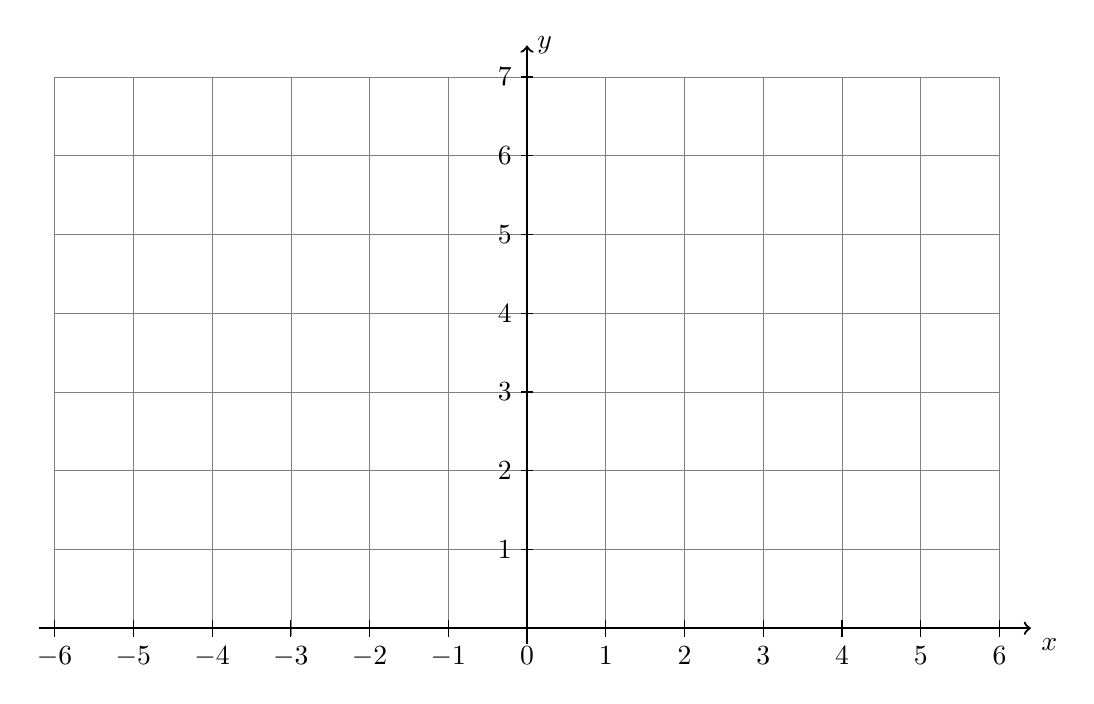
\begin{tikzpicture}[x=1cm, y=1cm, scale=1]
            \draw [help lines] (-6,-0.1) grid (6,7);
            \draw [thick, ->] (-6.2,0) -- (6.4,0) node [below right] {$x$};
            \draw [thick, ->] (0,-0.2)--(0,7.4) node [right] {$y$};
            \foreach \x in {-6,...,6}
                \draw[shift={(\x,0)}] (0,3pt)--(0,-3pt) node[below] {$\x$};
            \foreach \y in {1,...,7}
                \draw[shift={(0,\y)}] (2pt,0pt)--(-2pt,0pt) node[left]  {$\y$};
            \clip (-5,0) rectangle (5,5);
            %\draw [<->,thick,smooth,domain=-5:5] plot(\x,{(\x)^3+-4*(\x)^2-1*(\x)+4});
        \end{tikzpicture}
    \end{center}

\end{enumerate}
\end{document}



